I test eseguiti su Mole.io hanno privilegiato l'aspetto della raccolta dati operata dal sistema. Questa, infatti, � una delle principali funzionalit� offerte dall'applicazione ed � interessante comprendere come, l'ottimizzazione del layer di insertion, possa contribuire ad un incremento delle performance globali del sistema.

Durante i test sono state esplorate diverse configurazioni del database al fine di comprendere quale fosse la ottimale ai fini applicativi per Mole.io. I test sono stati eseguiti cercando di creare un ambiente il pi� possibile esente da fattori di incertezza esterni, al fine ottenere misure affidabili e risultati riproducibili.

Per lo svolgimento delle analisi, � stato realizzato un cluster MongoDB utilizzando tre \textit{virtual machine} (VM) rispettivamente configurate in modo da utilizzare 512 Megabyte di memoria RAM, con un Hard Disk SSD da 8,0 Gigabyte e dotate di un processore da 1,2 GHz. Ognuna delle VM � stata equipaggiata con una differente configurazione:
\begin{description}
\item[VM1] sulla quale sono stati installati un Query Router (\verb|mongos|), il cui compito � stato fornire l'accesso all'intero cluster e un Config Server (\verb|mongod|) opportunamente configurato per tenere traccia delle informazioni di \textit{layout} del cluster;
\item[VM2] su cui � stato installato il primo shard utilizzando un demone \verb|mongod|;
\item[VM3] clone della macchina precedente, necessaria per il secondo shard del cluster;
\end{description}

I test sono stati svolti utilizzando diverse configurazioni del cluster realizzato e misurando i tempi per l'inserimento di dati nel database. Per comprendere il significato delle diverse configurazioni del cluster, � necessario fare riferimento ad una nota, relativa alle chiavi di sharding, all'interno della documentazione di MongoDB:

\begin{quote}
\textit{When inserting documents with monotonically increasing shard keys, all inserts belong to the same chunk on a single shard. The system will eventually divide the chunk range that receives all write operations and migrate its contents to distribute data more evenly. However, at any moment the cluster can direct insert operations only to a single shard, which creates an insert throughput bottleneck.}
\end{quote}

Un requisito fondamentale di una buona chiave di sharding in MongoDB � la distribuzione probabilistica dei suoi valori. La documentazione di MongoDB, infatti, consiglia di utilizzare chiavi con una distribuzione di valori il pi� uniforme possibile, in modo da mantenere costante il carico di lavoro assegnato ad ogni shard. Da questo punto di vista, una buona chiave di sharding � l'id fornito automaticamente da MongoDB ad ogni documento.

Come � possibile leggere dalla citazione tratta dalla documentazione del database, per�, � fondamentale che le chiavi di sharding non utilizzino valori  monotoni, pena una riduzione significativa delle performance. Questo � dovuto al fatto che il balancer di MongoDB utilizza una logica di partizionamento basata sui valori delle chiavi. In presenza di valori con distribuzione monotona, il balancer non � in grado di eseguire un bilanciamento in tempo reale dei valori, e li salva sempre nell'ultimo shard disponibile, degradando le performance dell'intero cluster. L'\textit{id} fornito da MongoDB � generato a partire da un \textit{timestamp}, quindi, per costruzione, i valori degli id sono monotonicamente crescenti.

A fronte delle considerazioni precedenti, � stato scelto di eseguire i test utilizzando configurazioni del cluster differenziate sulla base della chiave di sharding scelta per bilanciare la base dati:
\begin{enumerate}
\item un solo shard, nessuna chiave di sharding;
\item due shard, utilizzando come chiave di sharding il campo \textit{id} fornito da MongoDB;
\item due shard, utilizzando come chiave il valore \textit{hash} del campo id, questo permette di ottenere, contemporaneamente, valori con distribuzione uniforme, non monotonicamente crescenti.
\end{enumerate}

I valori raccolti durante i test si riferiscono al tempo richiesto per inserire un numero definito di documenti all'interno del cluster. Sono stati utilizzati due tipi di documenti: \textit{small}, della dimensione di 200 byte circa, e \textit{big}, con una dimensione pari a 1 Megabyte. 

Per verificare la risposta del sistema al crescere del carico di lavoro richiesto, � stato creato uno script in grado di simulare un numero variabile di client (\textit{thread}). Ogni client esegue un numero prefissato di richieste di inserimento all'interno del database. 

Il numero dei client � stato fatto variare progressivamente da 1 a 100 con incrementi di 10. Il numero di richieste per client � stato impostato a 10 per i documenti di tipo \textit{big} e a 100 per i documenti di tipo \textit{small}. 

Le tabelle \ref{tab:benchmark-small} e \ref{tab:benchmark-big} riportano i risultati ottenuti, rispettivamente per i test eseguiti utilizzando documenti di tipo \textit{small} e \textit{big}. I valori riportati in tabella sono la media dei valori ottenuti da tre esecuzioni. I grafici \ref{fig:benchmark-small} e \ref{fig:benchmark-big} sono stati ottenuti ponendo sull'asse delle ascisse il numero dei client, e sull'asse delle ordinate il tempo richiesto dal cluster per l'inserimento di tutti i documenti del test.\\

\begin{table}[h]
\begin{center}
\begin{tabular}{r||r|r|r}
Client & 1 Shard & 2 Shard (id) & 2 Shard (hashed id) \\ 
\hline \hline 
1 & 0.239 & 0.172 & 0.285 \\
10 & 0.451 & 0.442 & 0.448 \\
20 & 0.884 & 0.909 & 0.983 \\
30 & 1.310 & 1.395 & 1.460 \\
40 & 1.776 & 1.859 & 1.960 \\
50 & 2.281 & 2.319 & 2.525 \\
60 & 2.751 & 2.862 & 3.112 \\
70 & 3.275 & 3.484 & 3.925 \\
80 & 3.798 & 3.910 & 4.525 \\
90 & 4.201 & 4.358 & 4.856 \\
100 & 4.784 & 4.967 & 5.604 \\
\end{tabular}
\caption{Risultati dei test con documenti \textit{small}}\label{tab:benchmark-small}
\end{center}
\end{table}

\begin{figure}[h]
\centering
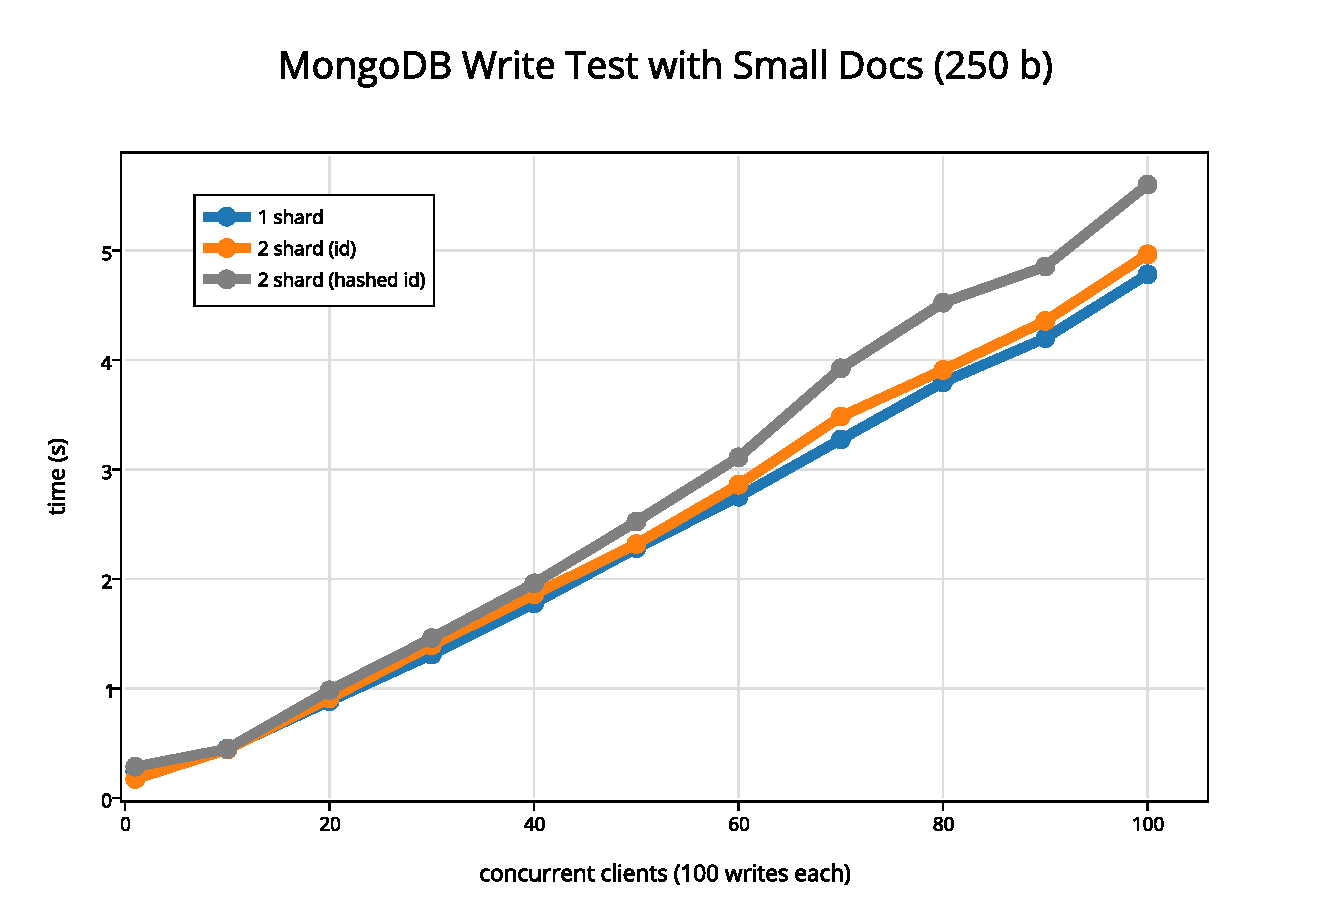
\includegraphics[width=1.0\linewidth]{./img/mongodb_write_test_with_small_docs_250_b}
\caption[Grafico dei risultati con documenti \textit{small}]{Grafico dei risultati con documenti \textit{small}}
\label{fig:benchmark-small}
\end{figure}

\begin{table}[h]
\begin{center}
\begin{tabular}{r||r|r|r}
Client & 1 Shard & 2 Shard (id) & 2 Shard (hashed id) \\ 
\hline \hline 
1 & 0.682 & 0.828 & 0.692 \\
10 & 2.165 & 2.853 & 2.095 \\
20 & 7.009 & 7.243 & 4.290 \\
30 & 8.753 & 10.141 & 6.335 \\
40 & 14.535 & 15.912 & 9.089 \\
50 & 31.931 & 43.645 & 12.949 \\
60 & 30.808 & 24.503 & 15.000 \\
70 & 46.350 & 59.534 & 19.179 \\
80 & 32.045 & 43.703 & 28.898 \\
90 & 114.287 & 97.787 & 25.843 \\
100 & 127.658 & 88.600 & 32.171 \\
\end{tabular}
\caption{Risultati dei test con documenti \textit{big}}\label{tab:benchmark-big}
\end{center}
\end{table}

\begin{figure}[h]
\centering
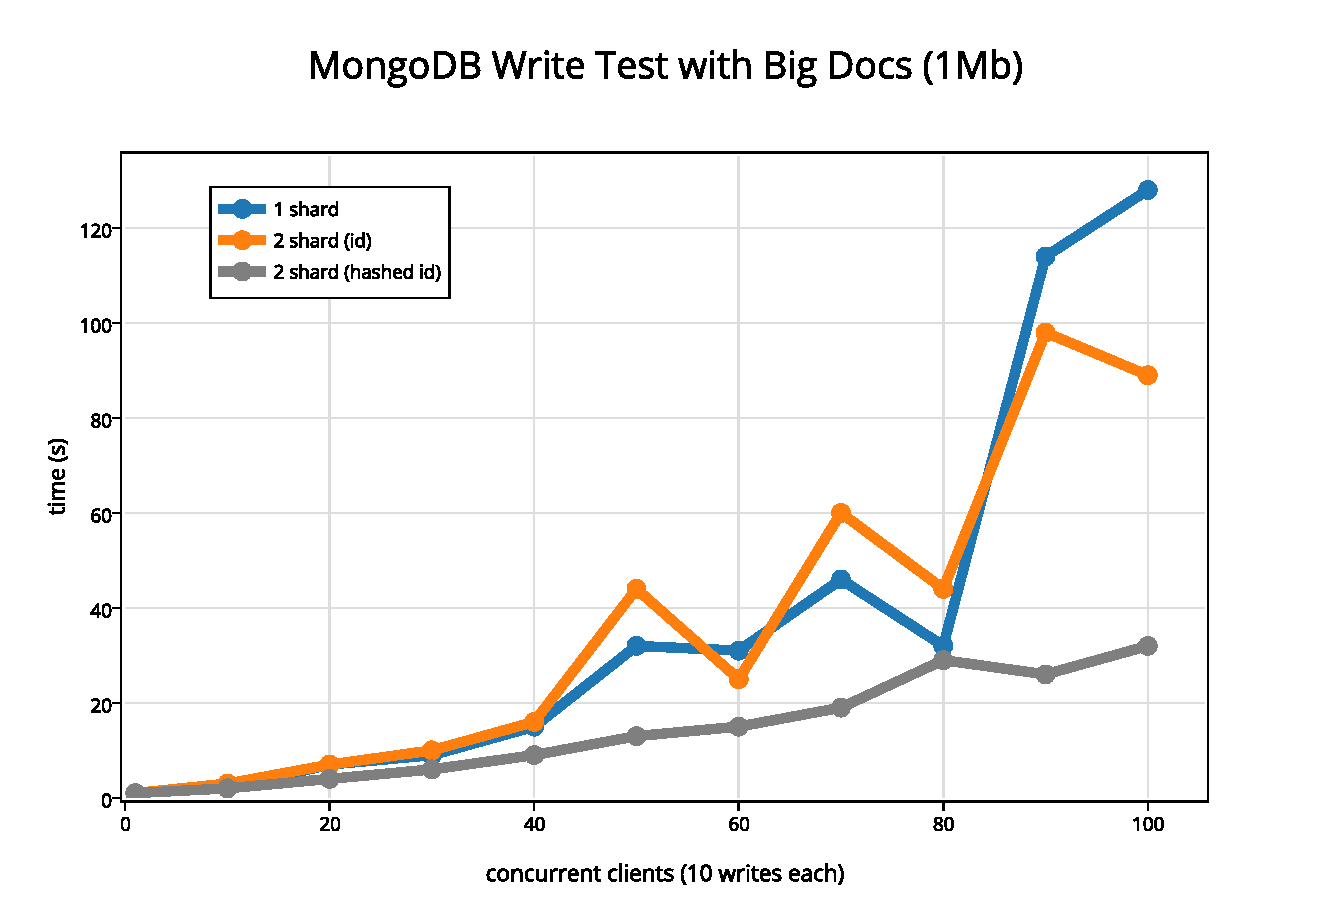
\includegraphics[width=1.0\linewidth]{./img/mongodb_write_test_with_big_docs_1mb}
\caption[Grafico dei risultati con documenti \textit{big}]{Grafico dei risultati con documenti \textit{big}}
\label{fig:benchmark-big}
\end{figure}

Osservando i risultati ottenuti � chiaro come lo sharding offra vantaggi concreti solo se la dimensione dei documenti da salvare � consistente. Il motivo di questo comportamento, risiede nella modalit� di lavoro del balancer e nella politica di gestione dei lock applicata da MongoDB.

Salvando documenti di piccole dimensioni su pi� shard, accade che il tempo richiesto dal write-lock � minimo e, di conseguenza non si arriva alla \textit{saturazione} delle code di scrittura del database. Scegliendo la politica di sharding che fa uso di hash, inoltre, il balancer � obbligato ad eseguire uno spostamento dei documenti a \textit{runtime}, degradando le performance rispetto alla scrittura su un singolo shard.

Nel caso di documenti di dimensioni maggiori, invece, l'\textit{overhead} aggiunto dal balancer � minimo rispetto al tempo di attesa dei documenti sulla coda di scrittura. Come conseguenza, si ottiene che l'utilizzo di pi� shard, e quindi di pi� code di scrittura parallele, aumenta notevolmente le performance dell'intero cluster.